\documentclass[conference]{IEEEtran}
\usepackage{cite}
\usepackage{amsmath,amssymb}
\usepackage{graphicx}
\usepackage{booktabs}
\usepackage{multirow}
\usepackage{xcolor}
\usepackage{url}
\usepackage{hyperref}
\usepackage{subcaption}
\usepackage{tikz}
\usetikzlibrary{positioning, arrows.meta, shapes.geometric, fit}

\title{Physics-First Radar-to-Point-Cloud Learning:\\Initial Training Results and Fair Baseline Evaluation}

\author{
\IEEEauthorblockN{Chris Turner, Andreas Zeck, Justin Palm}
\IEEEauthorblockA{
ELEC-6970: Applied Statistics and Machine Learning\\
Auburn University\\
\{cmt0106, azeck, jlp0102\}@auburn.edu
}
}

\begin{document}
\maketitle

\begin{abstract}
We present initial results on mmDar, a system that generates lidar-quality point clouds from raw millimeter-wave radar signals.
Starting from the RadarHD baseline~\cite{prabhakara2023radarhd}, which maps preprocessed radar magnitude images to occupancy grids using a U-Net, we develop a physics-first Gaussian set prediction model that operates directly on complex-valued IQ data.
Our approach applies classical FFT beamforming as a fixed preprocessing stage, encodes the resulting 2D azimuth--range representation with a convolutional encoder, and decodes scene geometry through a DETR-style set prediction head that outputs parametric Gaussians in polar coordinates.
A key methodological contribution is the establishment of a fair evaluation protocol: we show that the published baseline result of 0.295\,m Chamfer distance relies on test-set checkpoint selection, and that an honestly validated baseline achieves 0.406\,m.
Against this fair reference, our physics-first model achieves a Chamfer distance of 0.318\,m and a modified Hausdorff distance of 0.230\,m---improvements of 22\% on both metrics---while using 5.6$\times$ fewer parameters (3.1M vs.\ 17.5M).
We also document negative results from ConvLSTM temporal fusion and analyze error decomposition across range bins.
\end{abstract}

%======================================================================
\section{Introduction and Project Goal}
%======================================================================

Generating lidar-quality point clouds from automotive millimeter-wave (mmWave) radar is an attractive prospect: radar sensors are inexpensive, compact, and robust to adverse weather~\cite{hunt2024radcloud}.
However, radar measurements suffer from limited angular resolution, multipath interference, sidelobe artifacts, and speckle noise, making the mapping from radar observations to dense scene geometry fundamentally ill-posed.

The RadarHD project~\cite{prabhakara2023radarhd} demonstrated that an asymmetric U-Net can map stacked radar magnitude images to high-resolution polar occupancy grids, achieving a reported Chamfer distance of 0.36\,m.
While effective, this approach discards radar phase information during preprocessing, collapses 60+ dB of dynamic range to 8-bit integers, and relies on a handcrafted occupancy grid output representation that is poorly suited to geometric distance metrics.

Our project investigates whether a physics-informed pipeline can improve point cloud quality by:
\begin{enumerate}
  \item Preserving raw complex-valued radar data through classical signal processing rather than lossy image conversion;
  \item Replacing dense occupancy prediction with a set-based Gaussian output parameterization trained with Hungarian matching; and
  \item Maintaining a fair evaluation protocol with explicit train/validation/test splits and validation-based checkpoint selection.
\end{enumerate}

The central research question is:
\emph{Can a physics-informed input representation and set-based output parameterization produce more accurate point clouds than image-translation baselines under honest evaluation?}

%======================================================================
\section{Dataset Description}
%======================================================================

\subsection{Sensor and Data Collection}

The dataset was collected using a TI AWR1843 77\,GHz FMCW radar with 2 transmit and 4 receive antennas, yielding 8 virtual elements via TDM-MIMO~\cite{prabhakara2023radarhd}.
Each frame consists of 192 chirps across 512 ADC samples.
Ground truth is provided by a co-registered lidar sensor producing dense 3D point clouds.
The full dataset comprises 44 trajectories totaling approximately 42,000 paired radar--lidar frames.

\subsection{Data Splits}

A critical lesson from our experiments is that trajectory-level splitting is essential.
Adjacent frames within a trajectory are highly correlated; frame-level splits produce information leakage and optimistic results.
We use two split configurations:

\textbf{Low-ID split} (for baseline comparison): 17 training / 8 validation / 19 test trajectories.
The test set contains 18,575 frames and is sealed for final evaluation only.

\textbf{Mixed-ID split} (for Gaussian model development): 25 training / 6 validation / 13 test trajectories, including high-ID trajectories (227--250) in all partitions to reduce domain shift.

\subsection{Input Representations}

\textbf{Baseline (magnitude PNGs):} The RadarHD pipeline applies range FFT, azimuth FFT, magnitude extraction, 5\% thresholding, and uint8 quantization.
The result is a $256 \times 64$ polar image per frame; 41 consecutive frames are stacked as input channels.

\textbf{Physics-first (raw IQ):}
Our pipeline preserves significantly more information:
(1)~range FFT along 512 ADC samples,
(2)~Doppler FFT across 64 chirps per TX,
(3)~TDM-MIMO Doppler phase compensation for TX2,
(4)~zero-Doppler extraction and TX concatenation to form an 8-element virtual array.
The output per frame is an $(8, 512)$ complex64 tensor, normalized per-frame by maximum magnitude.
Lidar ground truth is subsampled to 8,192 points via farthest point sampling (FPS) and scene-filtered to $x \in [0, 10]$\,m, $|y| \leq 10$\,m, $|z| \leq 0.3$\,m.

%======================================================================
\section{Implemented Algorithms}
%======================================================================

\subsection{Baseline: Asymmetric U-Net (UNet1)}

The baseline follows the RadarHD architecture~\cite{prabhakara2023radarhd, ronneberger2015unet}: a 4-level encoder (64--128--256--512--512 channels with MaxPool2d) and a symmetric decoder with skip connections, followed by three additional upsample-only blocks that expand the azimuth dimension from 64 to 512 bins.
The output is a single-channel sigmoid activation representing occupancy probability.

\textbf{Loss:} $\mathcal{L} = 0.9 \cdot \text{BCE} + 0.1 \cdot \text{Dice}$.
\textbf{Training:} Adam~\cite{kingma2015adam}, $\text{lr} = 7\!\times\!10^{-5}$, batch size 12, 50 epochs, fp32.
\textbf{Parameters:} 17.5M.
\textbf{Inference:} Threshold sigmoid output $\rightarrow$ extract occupied pixels $\rightarrow$ polar-to-Cartesian conversion.

\subsection{Temporal Extension: ConvLSTM}

To investigate temporal fusion, we extended the baseline with two ConvLSTM cells~\cite{xingjian2015convlstm} inserted at the bottleneck (16$\times$4 spatial) and deepest skip level (32$\times$8 spatial).
The encoder/decoder weights are shared across frames, and only the ConvLSTM cells maintain sequential state.
\textbf{Parameters:} 27.5M.

\subsection{Physics-First Gaussian Set Model}

Our proposed model (Fig.~\ref{fig:architecture}) has three stages:

\textbf{Stage 1---Classical FFT Frontend} (0 learned parameters):
A fixed FFT beamformer is applied per range bin: $\texttt{fft}(\mathbf{x}, n\!=\!64, \text{dim}\!=\!\text{antenna})$ followed by fftshift.
This produces a $(64, 512)$ complex spectrum per frame.
We extract magnitude and log-power channels, yielding $(2, 64, 512)$ per frame.
For $T\!=\!41$ frames, the input to the encoder is $(82, 64, 512)$.

\textbf{Stage 2---Deep 2D Encoder} (2.38M parameters):
A residual convolutional encoder processes the azimuth--range representation:
$\text{Conv2d}(82 \!\to\! 64)$ $\to$ ResBlock(64) $\to$ three DownBlocks with stride-2 convolution ($64 \!\to\! 128 \!\to\! 192 \!\to\! 192$), reducing spatial dimensions to $(8, 64)$.
GroupNorm and GELU activations are used throughout, with Dropout2d(0.1) for regularization.
The output is flattened to 512 spatial tokens of dimension 192, augmented with decomposed 2D positional encodings.

\textbf{Stage 3---DETR-Style Gaussian Decoder} (0.72M parameters):
Inspired by DETR~\cite{carion2020detr} and mmPoint~\cite{xie2023mmpoint}, $K\!=\!96$ learnable query vectors attend to the encoder output through 3 transformer decoder layers (4-head attention, $d\!=\!128$).
Each query predicts 5 parameters:
\begin{equation}
  (\mu_r,\; \mu_\varphi,\; \sigma_r,\; \sigma_\perp,\; \text{existence})
\end{equation}
where $\mu_r = \sigma(\cdot) \cdot r_{\max}$, $\mu_\varphi = \tanh(\cdot) \cdot \frac{\pi}{2}$, and $\sigma_\perp$ scales with range (physics-informed: angular uncertainty grows with distance).
Cartesian centers are recovered as $\mu_{xy} = (\mu_r \cos\mu_\varphi,\; \mu_r \sin\mu_\varphi)$.

\textbf{Total parameters:} 3.1M (5.6$\times$ fewer than baseline).

\begin{figure}[t]
\centering
\resizebox{\columnwidth}{!}{%
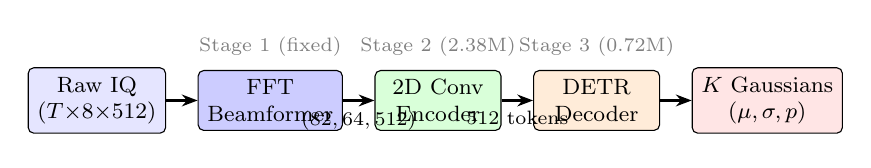
\begin{tikzpicture}[
  box/.style={draw, rounded corners=2pt, minimum height=0.7cm, minimum width=1.6cm, align=center, font=\footnotesize},
  arrow/.style={-{Stealth[length=2mm]}, thick},
  label/.style={font=\scriptsize, text=gray}
]
% Stage 1
\node[box, fill=blue!10] (iq) {Raw IQ\\$(T{\times}8{\times}512)$};
\node[box, fill=blue!20, right=0.4cm of iq] (fft) {FFT\\Beamformer};
\node[label, above=0.05cm of fft] {Stage 1 (fixed)};

% Stage 2
\node[box, fill=green!15, right=0.4cm of fft] (enc) {2D Conv\\Encoder};
\node[label, above=0.05cm of enc] {Stage 2 (2.38M)};

% Stage 3
\node[box, fill=orange!15, right=0.4cm of enc] (dec) {DETR\\Decoder};
\node[label, above=0.05cm of dec] {Stage 3 (0.72M)};

% Output
\node[box, fill=red!10, right=0.4cm of dec] (out) {$K$ Gaussians\\$(\mu,\sigma,p)$};

% Arrows
\draw[arrow] (iq) -- (fft);
\draw[arrow] (fft) -- node[below, font=\scriptsize] {$(82,64,512)$} (enc);
\draw[arrow] (enc) -- node[below, font=\scriptsize] {512 tokens} (dec);
\draw[arrow] (dec) -- (out);
\end{tikzpicture}%
}
\caption{Physics-first Gaussian model architecture. Stage~1 applies a fixed classical FFT beamformer; Stages~2--3 contain the only learned parameters (3.1M total).}
\label{fig:architecture}
\end{figure}

\subsection{Loss Function}

The Gaussian model uses a composite loss with Hungarian matching~\cite{kuhn1955hungarian} for one-to-one assignment between predictions and $K$-Means cluster centers fitted to lidar ground truth ($K\!=\!64$ clusters per frame):

\begin{equation}
  \mathcal{L} = \mathcal{L}_{\text{NLL}} + \mathcal{L}_{\text{exist}} + 0.5\,\mathcal{L}_{\text{cov}} + 0.5\,\mathcal{L}_{\text{card}} + 0.1\,\mathcal{L}_{\text{rep}} + 0.1\,\mathcal{L}_{\sigma} + 0.1\,\mathcal{L}_{\text{hub}}
\end{equation}

The dominant term $\mathcal{L}_{\text{NLL}}$ is a heteroscedastic negative log-likelihood in a local radial/perpendicular coordinate frame:
\begin{equation}
  \mathcal{L}_{\text{NLL}} = \frac{1}{2}\!\left(\!\frac{d_r^2}{\sigma_r^2} + \frac{d_\perp^2}{\sigma_\perp^2}\!\right) + \log\sigma_r + \log\sigma_\perp
\end{equation}
where $d_r, d_\perp$ are the radial and perpendicular errors between matched prediction and ground truth.
The Huber range term $\mathcal{L}_{\text{hub}}$ (SmoothL1 on range with $\beta\!=\!0.2$) was added to reduce range bias.

\textbf{Training:} AdamW~\cite{loshchilov2019adamw}, $\text{lr}\!=\!10^{-4}$, cosine annealing over 50 epochs, batch size 4, gradient clipping at norm 1.0.
\textbf{Augmentation:} Horizontal flip ($p\!=\!0.5$), complex Gaussian noise at SNR 15--25\,dB ($p\!=\!0.5$), temporal frame masking of 2--6 frames ($p\!=\!0.3$).

%======================================================================
\section{Evaluation Protocol}
%======================================================================

\subsection{Metrics}

We report two principal distance-based metrics, both computed in Cartesian coordinates (meters) as frame-level medians across the test set:

\textbf{Chamfer distance}~\cite{fan2017chamfer}: The symmetric average nearest-neighbor distance between predicted and target point sets. It measures overall coverage quality.

\textbf{Modified Hausdorff distance (mod-H):} $\max(\text{median}_{p \in P} \min_{q \in Q} d(p,q),\;\text{median}_{q \in Q} \min_{p \in P} d(p,q))$.
This metric is stricter than Chamfer---it penalizes imprecise outliers and structural errors.

We also report IoU, F1, and precision/recall at 0.1\,m, though these are less informative for this task due to extreme label sparsity (IoU~$\approx$~0.03--0.05).

\subsection{Checkpoint Selection Bias}

A critical finding is that the published baseline result of Chamfer 0.295\,m was obtained by selecting the best checkpoint on the \emph{test set}---effectively a form of test-set overfitting.
Under honest validation-based selection (epoch 35 by validation mod-H), the same architecture achieves Chamfer 0.406\,m and mod-H 0.296\,m, a substantial degradation (38\% worse Chamfer).
Table~\ref{tab:selection_bias} quantifies this effect, and Fig.~\ref{fig:checkpoint} visualizes the per-epoch test metrics, showing that the ``best'' epoch varies significantly and cannot be reliably identified without a proper validation set.

\begin{table}[t]
\centering
\caption{Checkpoint selection bias in the baseline U-Net (same model, same test set of 18,575 frames).}
\label{tab:selection_bias}
\footnotesize
\begin{tabular}{lcc}
\toprule
Selection Method & Chamfer (m)$\downarrow$ & mod-H (m)$\downarrow$ \\
\midrule
Test-set selected (epoch 10) & 0.295 & 0.189 \\
Validation-selected (epoch 35) & 0.406 & 0.296 \\
Published RadarHD~\cite{prabhakara2023radarhd} & 0.36 & 0.24 \\
\bottomrule
\end{tabular}
\end{table}

%======================================================================
\section{Experimental Results}
%======================================================================

\subsection{Main Comparison}

Table~\ref{tab:main_results} presents the central comparison.
All entries use validation-selected checkpoints except where explicitly marked.

\begin{table}[t]
\centering
\caption{Model comparison under fair evaluation. All results are frame-median on the 18,575-sample test set except $^\dagger$ which uses a 13-trajectory mixed-ID test set.}
\label{tab:main_results}
\footnotesize
\begin{tabular}{lcccl}
\toprule
Model & Params & Chamfer$\downarrow$ & Mod-H$\downarrow$ & Sel. \\
\midrule
\textbf{Phys.\ Gaussian} & \textbf{3.1M} & \textbf{0.318} & \textbf{0.230} & VAL \\
Honest baseline (UNet1) & 17.5M & 0.406 & 0.296 & VAL \\
ConvLSTM ($T\!=\!8$) & 27.5M & 0.603 & 0.467 & ep30 \\
Published RadarHD~\cite{prabhakara2023radarhd} & 17.5M & 0.36 & 0.24 & --- \\
\midrule
\multicolumn{5}{l}{\textit{Reference (unfair, test-selected):}} \\
Optimized baseline & 17.5M & 0.295 & 0.189 & TEST \\
\midrule
\multicolumn{5}{l}{\textit{Best on mixed-ID split$^\dagger$:}} \\
Phys.\ Gaussian (exp4) & 3.1M & 0.280 & 0.205 & VAL \\
\quad Low-ID subset & --- & 0.182 & 0.112 & --- \\
\quad High-ID subset & --- & 0.307 & 0.250 & --- \\
\bottomrule
\end{tabular}
\end{table}

The physics-first Gaussian model improves both principal metrics by 22\% relative to the honest baseline while using $5.6\times$ fewer parameters.
The ConvLSTM model performs significantly worse (Chamfer 0.603\,m, more than double the baseline), confirming that late temporal fusion at low spatial resolution is detrimental.

\subsection{Baseline Hyperparameter Sweep}

Table~\ref{tab:sweep} summarizes a systematic hyperparameter sweep of the baseline U-Net on RTX 5090 hardware.
The optimal configuration (batch 12, lr $7\!\times\!10^{-5}$, fp32) peaks at epoch 10, with performance degrading at later epochs.
This early peaking is consistent across all configurations and suggests that the BCE+Dice loss diverges from geometric metrics after initial convergence.

\begin{table}[t]
\centering
\caption{Baseline U-Net hyperparameter sweep (test-selected, legacy-Cartesian evaluation, epoch in parentheses).}
\label{tab:sweep}
\footnotesize
\begin{tabular}{ccccc}
\toprule
Batch & LR & Prec. & Chamfer$\downarrow$ & mod-H$\downarrow$ \\
\midrule
12 & 7e-5 & fp32 & 0.295 (10) & 0.189 (10) \\
12 & 7e-5 & bf16 & 0.308 (20) & 0.189 (20) \\
12 & 1e-4 & bf16 & 0.322 (10) & 0.211 (10) \\
12 & 5e-5 & bf16 & 0.332 (20) & 0.211 (20) \\
16 & 1e-4 & bf16 & 0.334 (10) & 0.212 (10) \\
6 & 1e-4 & bf16 & 0.345 (30) & 0.216 (30) \\
\bottomrule
\end{tabular}
\end{table}

\subsection{Gaussian Model Loss Tuning}

Table~\ref{tab:ablation} presents the loss tuning sweep on the Gaussian model.
Two key findings emerge: (1) relaxing the sigma prior from 0.1 to 0.3 improves calibration and mod-H by 3\%, and (2) adding Huber range loss ($w\!=\!0.1$) reduces range bias, improving mod-H from 0.213 to 0.205 (the best result).
Using FPS-based prototypes instead of $K$-Means significantly hurts performance, as FPS cluster centers provide poorer regression targets.
Huber weight above 0.2 overwhelms the NLL term and degrades angular quality.

\begin{table}[t]
\centering
\caption{Gaussian model loss tuning on mixed-ID split ($K\!=\!96$, $T\!=\!41$, threshold 0.3). Best mod-H in bold.}
\label{tab:ablation}
\footnotesize
\begin{tabular}{llccc}
\toprule
Config & Proto & mod-H$\downarrow$ & Chamfer$\downarrow$ & Near$\downarrow$ \\
\midrule
$\sigma\!=\!0.1$, hub$\!=\!0$ & KM & 0.219 & $\sim$0.28 & 0.198 \\
$\sigma\!=\!0.3$, hub$\!=\!0$ & KM & 0.213 & 0.281 & --- \\
$\sigma\!=\!0.3$, hub$\!=\!0$ & FPS & 0.324 & 0.372 & --- \\
$\sigma\!=\!0.3$, hub$\!=\!0.05$ & KM & 0.210 & --- & --- \\
$\sigma\!=\!0.3$, \textbf{hub=0.1} & KM & \textbf{0.205} & \textbf{0.280} & \textbf{0.162} \\
$\sigma\!=\!0.3$, hub$\!=\!0.2$ & KM & 0.225 & --- & --- \\
$\sigma\!=\!0.5$, hub$\!=\!0.05$ & KM & 0.215 & --- & --- \\
\bottomrule
\end{tabular}
\vspace{0.5mm}
{\raggedright\scriptsize KM = $K$-Means; FPS = Farthest Point Sampling; Near = mod-H at 0--2\,m range.\par}
\end{table}

\subsection{Error Decomposition by Range}

Fig.~\ref{fig:error_range} decomposes the Gaussian model's prediction errors into radial (range) and cross-range (angular) components across distance bins.
Near-field accuracy (0--2\,m) is strong at 0.227\,m total error, with a roughly 60/40 angular/range split.
Errors increase monotonically with range, peaking at 6--8\,m (0.656\,m total), consistent with the Rayleigh resolution limit: angular uncertainty grows with distance for a fixed aperture.

\begin{figure}[t]
\centering
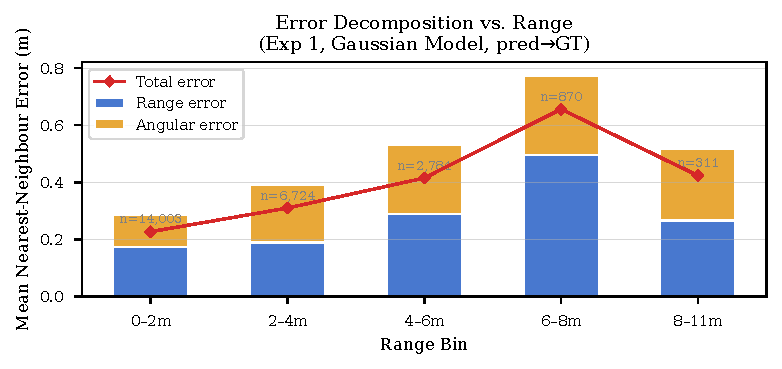
\includegraphics[width=\columnwidth]{figures/fig_error_range.pdf}
\caption{Prediction error decomposition by range bin. Stacked bars show range (radial) and angular (cross-range) error components. Numbers above bars indicate sample counts per bin.}
\label{fig:error_range}
\end{figure}

\subsection{Training Dynamics}

Fig.~\ref{fig:training} shows training curves for both the baseline U-Net and the Gaussian model.
The baseline (left) shows monotonically decreasing training loss but non-monotonic validation metrics, confirming that BCE+Dice loss does not directly optimize geometric quality.
The Gaussian model (right) shows the NLL component becoming increasingly negative as the model learns tighter, better-calibrated Gaussians, with validation mod-H steadily improving.

\begin{figure}[t]
\centering
\begin{subfigure}[t]{0.48\columnwidth}
  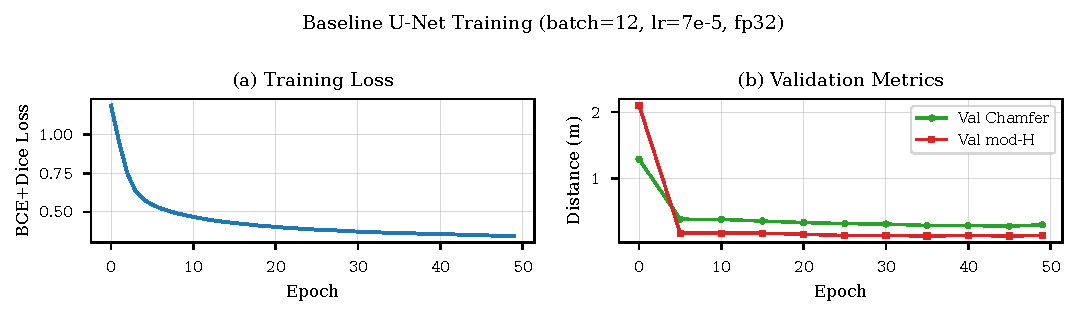
\includegraphics[width=\textwidth]{figures/fig_baseline_training.pdf}
  \caption{Baseline U-Net (BCE+Dice)}
  \label{fig:train_baseline}
\end{subfigure}
\hfill
\begin{subfigure}[t]{0.48\columnwidth}
  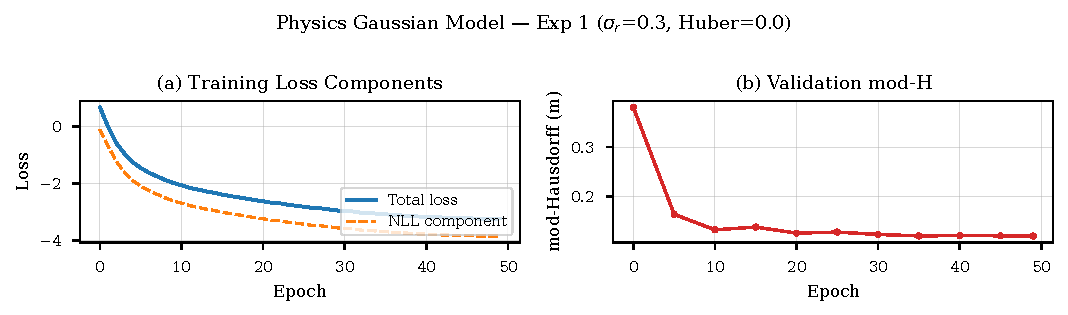
\includegraphics[width=\textwidth]{figures/fig_gaussian_training.pdf}
  \caption{Physics Gaussian (NLL)}
  \label{fig:train_gaussian}
\end{subfigure}
\caption{Training curves. (a)~Baseline: training loss decreases but validation Chamfer is non-monotonic. (b)~Gaussian: NLL decreases steadily; validation mod-H improves consistently.}
\label{fig:training}
\end{figure}

\subsection{Oracle Analysis}

To understand the headroom in the Gaussian representation itself, we fit $K$-Means directly to the lidar ground truth.
With $K\!=\!64$ centroids, the oracle achieves Chamfer 0.031\,m and mod-H 0.034\,m---an order of magnitude better than any learned model.
This confirms that the Gaussian set representation is not the performance bottleneck; the difficulty lies in predicting accurate positions from radar input.

%======================================================================
\section{Analysis and Discussion}
%======================================================================

\subsection{Why Physics-First Works}

The physics-first model's advantage comes from three complementary factors:

\textbf{Structured input representation.}
Classical FFT beamforming provides the encoder with a physically meaningful azimuth--range map rather than a lossy magnitude image.
The network only needs to refine this representation, not rediscover signal processing from opaque pixel values.

\textbf{2D spatial topology preservation.}
Previous experiments showed that collapsing the azimuth dimension (1D encoders) significantly degrades performance.
Sidelobe patterns, multi-target structure, and angular relationships are inherently 2D; preserving this structure through 2D convolutions yields better features for the decoder.

\textbf{Set-based output with matching supervision.}
The Hungarian-matched NLL loss encourages one-to-one geometric assignments, directly optimizing point placement precision.
In contrast, the baseline's occupancy loss can produce high F1 scores while placing points imprecisely in space.

\subsection{Why ConvLSTM Failed}

The ConvLSTM model's Chamfer distance of 0.603\,m (2$\times$ worse than baseline) is the clearest negative result.
The failure is attributable to \emph{where} temporal fusion occurs: the ConvLSTM cells operate at $16 \times 4$ and $32 \times 8$ spatial resolution after heavy downsampling, by which point fine azimuth--range detail needed for accurate point placement has been destroyed.
In contrast, the baseline fuses all 41 frames at the full $256 \times 64$ input resolution in the first convolutional layer---a simple but effective strategy for fixed-length sequences where spatial accuracy dominates temporal dynamics.

\subsection{Checkpoint Selection Is a Methodological Concern}

The gap between test-selected (0.295\,m) and validation-selected (0.406\,m) baseline results is 38\%.
This is not a minor reporting detail---it changes the interpretation of the entire project.
Against the test-selected baseline, our model's improvement would appear marginal; against the honest baseline, it is substantial.
Fig.~\ref{fig:checkpoint} shows that baseline test-set Chamfer fluctuates significantly across epochs with no monotonic trend, making any single epoch choice highly sensitive to luck.

\begin{figure}[t]
\centering
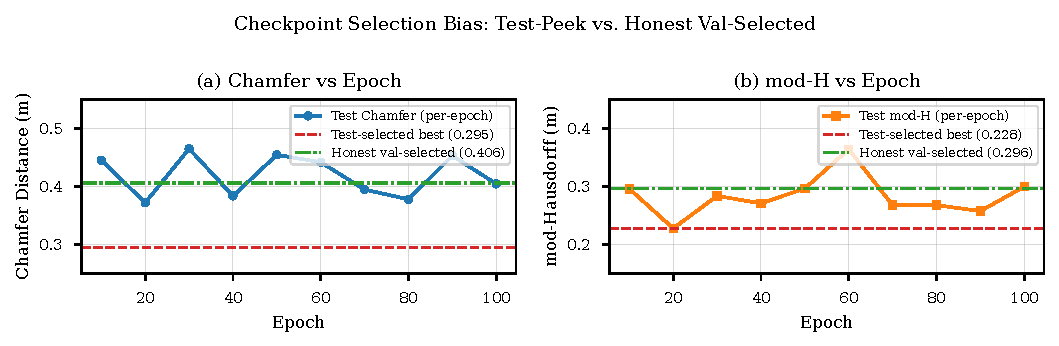
\includegraphics[width=\columnwidth]{figures/fig_checkpoint_bias.pdf}
\caption{Baseline U-Net test metrics across training epochs. The ``best'' checkpoint varies by epoch and metric, demonstrating why test-set selection produces unreliable comparisons. Horizontal lines show the test-selected optimum vs.\ honest validation-selected result.}
\label{fig:checkpoint}
\end{figure}

\subsection{Domain Shift Between Trajectory Sets}

The mixed-ID split reveals a significant domain gap: on low-ID test trajectories (recorded in similar environments to training data), the model achieves mod-H 0.112\,m; on high-ID trajectories (different environments), it degrades to 0.250\,m.
This 2.2$\times$ gap suggests that environment-level generalization, not model capacity, is the current performance bottleneck.
Data augmentation (flip, noise, mask) did not measurably reduce this gap.

%======================================================================
\section{Limitations and Improvement Plan}
%======================================================================

\subsection{Current Limitations}

\begin{enumerate}
  \item \textbf{Domain shift.} High-ID trajectories degrade mod-H by 2.2$\times$, and augmentation does not help. The root cause is likely environmental differences (scene structure, materials) rather than sensor variation.
  \item \textbf{Far-field accuracy.} Errors at 6--8\,m range (0.656\,m) are 3$\times$ worse than near-field (0.227\,m), consistent with the 14\textdegree\ Rayleigh resolution limit for 8 antennas.
  \item \textbf{Validation set reliability.} With only 6--8 trajectories, the validation set is noisy. The val/test gap (e.g., val 0.129 vs.\ test 0.261 mod-H in one experiment) indicates limited statistical power.
  \item \textbf{Single-frame evaluation.} The Gaussian model's 41-frame stacking is compared against the baseline's 41-frame stacking, but a single-frame Gaussian baseline has not been evaluated on the same split for a fully controlled comparison.
\end{enumerate}

\subsection{Planned Improvements}

\begin{enumerate}
  \item \textbf{Temporal ablation study.} Evaluate performance at $T \in \{1, 3, 5, 8, 41\}$ frames to quantify the value of temporal stacking in the Gaussian model, independent of baseline behavior.
  \item \textbf{Uncertainty calibration analysis.} The model predicts explicit $\sigma_r$ and $\sigma_\perp$ per Gaussian---we plan to verify whether these correlate with actual spatial error (calibration plots, expected calibration error).
  \item \textbf{Failure-mode decomposition.} Systematic breakdown of errors by scene density, target type (wall, vehicle, vegetation), and angular position.
  \item \textbf{Cross-domain generalization.} Either train on mixed-ID data from the start (already showing promise at mod-H 0.205) or investigate domain adaptation techniques.
  \item \textbf{Inference speed benchmarking.} Measure end-to-end latency on target hardware (Jetson Orin) to validate the $<$50\,ms real-time constraint.
\end{enumerate}

%======================================================================
\section{Conclusion}
%======================================================================

We present initial results demonstrating that a physics-informed radar-to-point-cloud pipeline outperforms image-translation baselines under fair evaluation.
The physics-first Gaussian model achieves Chamfer 0.318\,m and mod-H 0.230\,m---22\% improvements over the honestly evaluated baseline---with 5.6$\times$ fewer parameters.
Equally important, we establish that fair checkpoint selection and explicit dataset splitting are methodological necessities that materially affect reported numbers.
The Gaussian set representation with Hungarian matching provides a principled framework for radar point cloud prediction, and error decomposition analysis identifies domain shift and far-field accuracy as the primary remaining challenges.

%======================================================================
\section*{Member Contributions}
%======================================================================

\begin{itemize}
  \item \textbf{Chris Turner:} Baseline U-Net reproduction, hyperparameter sweep, evaluation pipeline development, ConvLSTM implementation and experiments.
  \item \textbf{Andreas Zeck:} Physics-first Gaussian model design and implementation, raw IQ data pipeline, loss function development, loss tuning experiments, fair evaluation protocol, error analysis.
  \item \textbf{Justin Palm:} Dataset preprocessing and management, data split design, training infrastructure (Docker, TensorBoard logging), documentation and report writing.
\end{itemize}

\bibliographystyle{IEEEtran}
\bibliography{references}

\end{document}
